% !TeX program = lualatex
% !TeX root = main.tex

\chapter{Introduction}
\emph{%
This chapter contains the general motivation, followed by the problem statement and concludes with an overview of the thesis structure.
}\label{chap:intro}
%

\section{Motivation}
On the brink of the millennium, several important developments were happening, which have led to today's massive amount of user generated content, often containing precise location (geotagged) data.

%GPS
The evolution of the American navigation satellite system GPS (Global Positioning System), together with the growing usage in the civil sector led in 2000 to the disabling of SA (selective availability). SA added intentional varying errors to the publicly receivable signal, distorting the location data up to 100 meters.
%, in fear of abusing the technique against America, e.\,g. in guided missiles. 
Today, the accuracy of GPS is up to 15 meters. Many organizations are working on systems similar to GPS, enabling locally better results, and to be not depended on GPS alone, for example the Galileo positioning system by the European Union.

%web 2.0
Big improvements were been done in web technologies like HTML and JavaScript, leading to a tremendous change in the perception of the internet -- gathering information was not any more the only thing you could do. Web 2.0 invited the users to participate, to create and share information themselves. Platforms like Wikipedia or Flickr are good examples for the spirit of this movement. 

Finally the miniaturization of processor chips created fast mobile phone computers -- smart phones -- at affordable prices. The resulting omnipresence of these smart phones, together with integrated GPS sensors and wireless internet connectivity whenever the user wishes creates the massive amount of user generated geotagged data. Many different internet platforms\,/\,services exist, most of them offering programming interfaces for mining the data, thus enabling interested people the possibility to analyse the data. 

This data openness can also bring dangers to individuals, by publishing too much or too sensitive data. Potential dangers include stalking\,/\,observation, identity theft and general scamming. To minimize these threads there is a need for more internet safety and awareness education, especially in schools, stricter out-of-the-box configuration of consumer ware and better security of the internet platforms saving the personal information.

Aside from these potential negative effects, users obviously wish to use these services, resulting in manifold use cases for this data, like recommender systems, event detection, news extraction and disaster management.

For example \textcite{Cheng2011} used 22 million check-ins (spatial temporal data points) from 220\,000 users of location sharing services like Foursquare, Twitter and Facebook Places in order to analyse human mobility patterns. The distance between consecutive check-ins, the deviation of distances between the users center of mass and the check-ins, and the probability of returning to distinctive points were among the investigated topics. Their results concluded that the users of these services have periodic behaviours and that geographic respectively economic constraints, together with individual social status, affect mobility patterns.

Beautiful and meaningful visualizations are also possibly as seen in figure~\ref{fig:twitter_london}. \textcite{Cheshire2012} collected twitter data over the summer period of 2012 around the Olympic Park in London and plotted the 3.3~million tweets coloured after the language detected. Grey (English) obviously dominates, but there are very clear accumulations in other colours like red (French), green (Arabic) and blue (Turkish).

\begin{figure}%[ht]
\centering
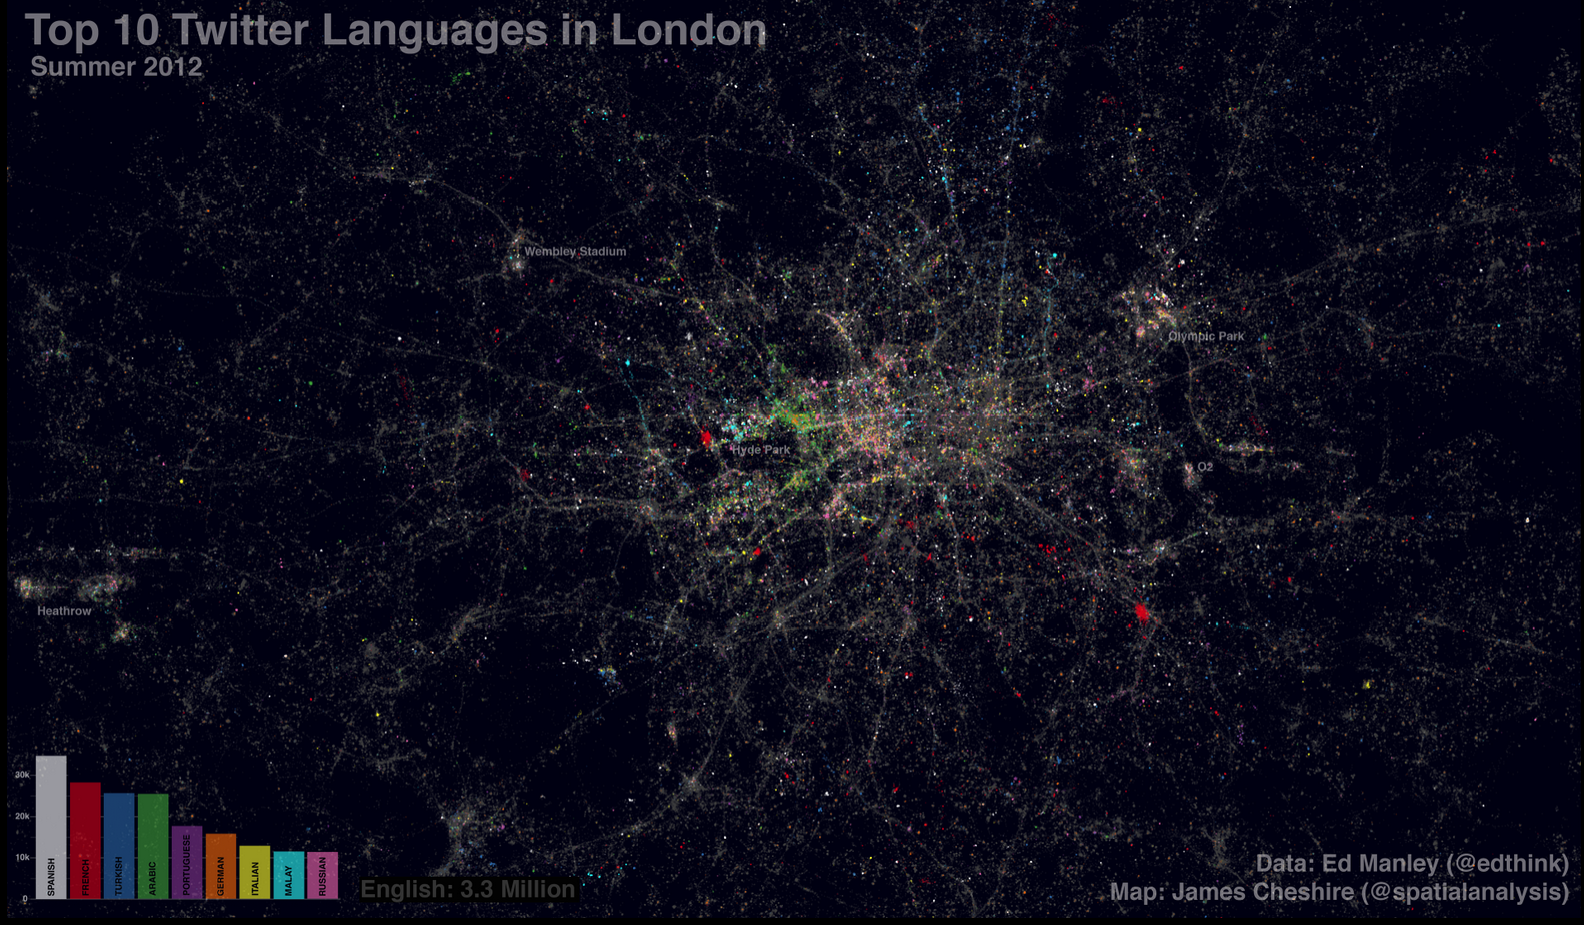
\includegraphics[width=\textwidth]{pix/twitter_lang_london.png}
\caption[Twitter Languages in London]{Twitter Languages in London\cite{Cheshire2012}}
\label{fig:twitter_london}
\end{figure}

These accumulations can be interpreted as geographical topics. \enquote*{A geographical topic is a spatially coherent meaningful theme. In other words, the words that are often close in space are clustered in a topic.}\cite{Yin2011} Geographical topic discovery has several use cases.\cite{Sizov2010} Companies offering free web-services can employ them very efficient because of their vast capacities and unfiltered access (if they have many active users).
\begin{description}
\item[Content organization] Modern cameras (especially mobile phone cameras) have the ability to save each photo with the location where it was taken. By using the location data the photos can be automatically categorized, or filtering when later searching for specific pictures of a landmark. Annotations and tags can be applied based on location,  direction and content of the photos.

\item[Search with spatial awareness]
Search engines can leverage additional spatial data, like GPS locations or keywords, to refine the search results. 

For example when searching for a restaurant with a mobile phone, the search application can either automatically commit the GPS data, or filter the results of the search engine based on it; without explicit knowledge of the user.

\item[Tag recommendation]% and exploration]
This use case is similar to the first example with photo annotations based on the location. Different specific locations can be recommended based on the given keywords.

For example when searching for the next holiday location and typing  \enquote{sun, beach, europe}, recommendations for further keywords could either be Nice (France), Crete (Greece) or Tenerife (Spain).

\item[Targeted advertisement]
Companies can optimize their strategies whether they should spend money on advertisement in regions where their product is already well known, or if they should rather advertise in other regions with similar geographic features, but less sales.
\end{description}
%
Besides these search, recommendation and exploration uses, geographic topics can also be used as early-warning system if timestamps are used. Various works explore these cases, mostly Twitter related for its active community and real time streaming API\cite{Vieweg2010, Mendoza2010, Hughes2009}.


\section{Problem Statement}
Using a dataset $D = \{d_1, \dots, d_n\}$ of geo-tagged documents $d_i = {text_i, location_i}$, and a cluster algorithm, meaningful geographic topics have to be found with a distance function based on a graph algorithm, which incorporates $text_i$ and $location_i$. The baseline compare function is composed of a naive linear combination of distance functions using $text_i$ and $location_i$ on vector representations of the data.

Extensive quantitative and qualitative evaluation of the results of these distance functions will be done done, using standard cluster evaluation measures with real world datasets. Evaluation includes the performances of the distance functions, as well as the performance of the evaluation measures in distinguishing between good and bad geographic topic results.

\vspace{.5em}
\noindent
As seen later in related works, evaluations are usually with rather small datasets, in contrast to the constant reminders of growing datasets. Datasets labelled with a ground truth (telling how the documents should be grouped) are evaluated using standard methods, but their datasets are small. If there are quantitative evaluations employed, on the small datasets, the comparison to different works is very hard to make.

Contributions of this thesis are the deployment of an extensible graph algorithm for finding geographical topics and its comparison to a naive baseline. And the consideration of cluster evaluation measures for quantitative evaluation of geographic topics with massive datasets containing more than one million points.

\vspace{.5em}
\noindent
The remaining thesis is structured as follows:

Chapter~\ref{chap:topics} introduces the general concepts of geographical topic models, clustering and lists the related works. Afterwards in chapter~\ref{chap:cluster} the used clustering algorithm is presented, and the used baseline distance function is motivated. Chapter~\ref{chap:graph} gives a general introduction to graphs and graph based algorithms, followed by a presentation of the graph-based approach by \textcite{Zhou2009} alongside some implementation adoptions. An explanation of the graph generation from the datasets concludes this chapter. Finally chapter~\ref{chap:eval} begins with a description of the different used evaluation metrics together with examples about their strengths and weaknesses. Subsequently the used datasets are introduced and the choice of parameters is discussed. The resulting comparison between the vector- and graph-based approaches with quantitative and qualitative evaluations leads directly to the conclusion of the thesis with a summery and future work in chapter~\ref{chap:future}.




%\section{Thesis Goals}
%Searching (and finding) such accumulations (clusters) among millions of points is called \emph{clustering}. Clustering is a common technique, with many different approaches, whose aim is to group similar objects together. Similarity is usually defined as distance, where smaller values indicate greater affinity.
%
%
%Geo-tagged data has a natural similarity measure among points, which is the distance $d_{location}$ between the locations from where the data has been transmitted. Clustering using this similarity measure can be interesting, but can be more interesting and meaningful if combined with other information. For example figure~\ref{fig:twitter_london} would be less than half as intriguing without the language information.
%
%This language information can be seen as a form of \emph{topic}. A topic is generally seen as a combination of words\,/\,sentences or other useful information describing or forming an abstract idea or general meaning. Using figure~\ref{fig:twitter_london} again, every tweet containing words or sentences have had their topic assigned as the recognized language of those words or sentences. It is clear that the process of finding such topics is heavily dependent on the used data and the use case for those topics.
%
%A simple form of topic detection is clustering the data points with a distance $d_{topic}$ based on processing the words or sentences contained in the data points. Every cluster can then seen as a topic, described by the contained words and their frequencies.
%
%Combining these two leads to \emph{geographical topic detection}. This task aims at providing useful regional topics.
%
%
%
%Using vector-based distance measures for text\,/\,topic distance $d_{topic}$ and geographical distance $d_{location}$, a combined distance $\alpha \, d_{topic} + \beta \, d_{location} = d_{combined}$ can be used to cluster both geographical and topical close objects, hopefully resulting in useful regional topics.
%
%\vspace{1em}
%\noindent
%Another approach is by performing abstractions. A graph can be a useful abstraction in working with objects having some sort of relationship with each other. A graph consists of nodes (objects), edges between those nodes (relationships) and attributes on either nodes or edges (features\,/\,weights). The affinity between objects in terms of text\,/\,topic distance and geographical distance will be represented by edges and weights.
%
%An example of a graph is a street map. Nodes are different cities, villages or other travelling targets. Edges are the streets connecting them, which represents the relationship of being able to travel from one point of interest to the next. Attributes are the names of the cities, or the speed limit of the streets. Defining the distance between two cities (nodes) can now be done based on the different streets (edges), for example the shortest\,/\,fastest route, the number of routes with maximal distance or travelling time and so on.
%
%For the task of identifying geographical topics a graph-based distance measure $d_{graph}$ will be used, which basically counts the number of possible routes between two nodes within a maximum length of these routes\cite{Zhou2009}. The higher the count the nearer\,/\,more similar the nodes are.
%
%
%
%
%\vspace{1em}
%\noindent
%This graph-based distance approach will be extensively compared to the above vector-based clustering with combined distances. In order to accomplish that, the clustering algorithm DBSCAN will be introduced in chapter~\ref{chap:cluster} together with the vector-based text and geographical distances.
%
%Chapter~\ref{chap:graph} explains the generation of the graphs from the datasets, followed by a presentation of the graph-based approach by \textcite{Zhou2009} alongside implementation adoptions.  
%
%Finally chapter~\ref{chap:eval} about the evaluation begins with describing the different used evaluation metrics and datasets. The resulting comparison between the vector- and graph-based approaches comes next, followed by the conclusion of the thesis with a summery and future work.
%
%\todo{Problem Statement}
%\todo{Contributions}